\documentclass[residuals.tex]{subfiles}
\begin{document}
\Large

\section{Regression Deletion Diagnostics}

This suite of functions can be used to compute some of the regression (leave-one-out deletion) diagnostics for linear and generalized linear models discussed in Belsley, Kuh and Welsch (1980), Cook and Weisberg (1982), etc.

\subsection*{Details}
\begin{itemize}
	\item The primary high-level function is \texttt{influence.measures} which produces a class "infl" object tabular display showing the DFBETAS for each model variable, DFFITS, covariance ratios, Cook's distances and the diagonal elements of the hat matrix. Cases which are influential with respect to any of these measures are marked with an asterisk. 
	
	\item The functions \texttt{dfbetas}, \texttt{dffits}, \texttt{covratio} and \texttt{cooks.distance} provide direct access to the corresponding diagnostic quantities. 
	
	\item Functions \texttt{rstandard} and \texttt{rstudent} give the standardized and Studentized residuals respectively. 
	( Definition here is different )
	\item (These functions re-normalize the residuals to have unit variance, using an overall and leave-one-out measure of the error variance respectively.) 
	
	\item Values for generalized linear models are approximations, as described in Williams (1987) (except that Cook's distances are scaled as F rather than as chi-square values). The approximations can be poor when some cases have large influence. 
	
	\item The optional i\texttt{nfl}, \texttt{res} and \texttt{sd} arguments are there to encourage the use of these direct access functions, in situations where, e.g., the underlying basic influence measures (from \texttt{lm.influence} or the generic influence) are already available. 
	
	\item Note that cases with \texttt{weights == 0} are dropped from all these functions, but that if a linear model has been fitted with \texttt{na.action = na.exclude}, suitable values are filled in for the cases excluded during fitting. 
	
	\item 
	The function \texttt{hat()} exists mainly for S (version 2) compatibility; we recommend using \texttt{hatvalues()} instead. 
\end{itemize}
 

\begin{framed}
	\begin{verbatim}
	Usage
	influence.measures(model)
	
	rstandard(model, ...)
	
	## S3 method for class 'lm'
	rstandard(model, infl = lm.influence(model, do.coef = FALSE),
	sd = sqrt(deviance(model)/df.residual(model)), ...)
	
	## S3 method for class 'glm'
	rstandard(model, infl = influence(model, do.coef = FALSE),
	type = c("deviance", "pearson"), ...)
	\end{verbatim}
\end{framed}

%==================================================== %
\begin{framed}
	\begin{verbatim}
	rstudent(model, ...)
	
	## S3 method for class 'lm'
	rstudent(model, infl = lm.influence(model, do.coef = FALSE),
	res = infl$wt.res, ...)
	
	## S3 method for class 'glm'
	rstudent(model, infl = influence(model, do.coef = FALSE), ...)
	
	dffits(model, infl = , res = )
	\end{verbatim}
\end{framed}
\newpage
\section{Influential Points in Regression}
% - http://stattrek.com/regression/influential-points.aspx
 

%ometimes in regression analysis, a few data points have disproportionate effects on the slope of the regression equation. In this lesson, we describe how to identify those influential points.


\begin{figure}
\centering
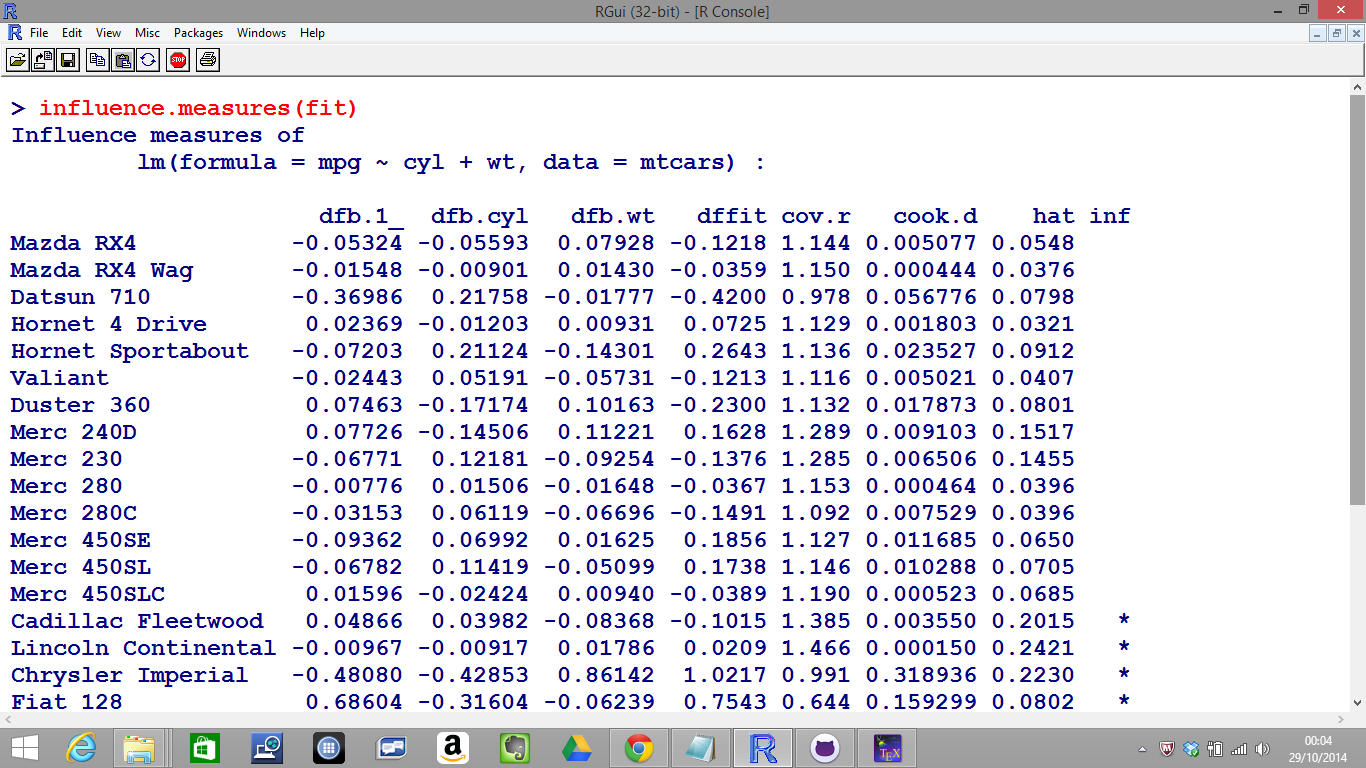
\includegraphics[width=1.1\linewidth]{Screenshot2}
\caption{}
\label{fig:Screenshot2}
\end{figure}


\begin{verbatim}
inflm.fit <- influence.measures(fit)
which(apply(inflm.fit$is.inf, 1, any))
\end{verbatim}
%-------------------------------------------------------------------------------------------%
\newpage


%==================================================== %
\begin{framed}
	\begin{verbatim}
	dfbeta(model, ...)
	## S3 method for class 'lm'
	dfbeta(model, 
		infl = lm.influence(model, do.coef = TRUE), ...)
	
	dfbetas(model, ...)
	
	## S3 method for class 'lm'
	dfbetas(model, 
		infl = lm.influence(model, do.coef = TRUE), ...)
	
	covratio(model, 
		infl = lm.influence(model, do.coef = FALSE),
	res = weighted.residuals(model))
	\end{verbatim}
\end{framed}

%==================================================== %
\begin{framed}
	\begin{verbatim}
	cooks.distance(model, ...)
	## S3 method for class 'lm'
	cooks.distance(model, 
		infl = lm.influence(model, do.coef = FALSE),
	res = weighted.residuals(model),
	sd = sqrt(deviance(model)/df.residual(model)),
	hat = infl$hat, ...)
	
	## S3 method for class 'glm'
	cooks.distance(model, 
		infl = influence(model, do.coef = FALSE),
	res = infl$pear.res,
	dispersion = summary(model)$dispersion,
	hat = infl$hat, ...)
	\end{verbatim}
\end{framed}

%==================================================== %
\begin{framed}
	\begin{verbatim}
	hatvalues(model, ...)
	## S3 method for class 'lm'
	hatvalues(model, 
		infl = lm.influence(model, do.coef = FALSE), ...)
	
	hat(x, intercept = TRUE)
	
	\end{verbatim}
\end{framed}
\newpage
\begin{verbatim}
Arguments
model an R object, typically returned by lm or glm.

infl influence structure as returned by lm.influence or influence (the latter only for the glm method of rstudent and cooks.distance).

res (possibly weighted) residuals, with proper default.

sd standard deviation to use, see default.

dispersion dispersion (for glm objects) to use, see default.

hat hat values H[i,i], see default.

type type of residuals for glm method for rstandard.

x the X or design matrix.

intercept should an intercept column be prepended to x?

... further arguments passed to or from other methods.

\end{verbatim}

%========================================================================================== %
\newpage




\end{document}


